\documentclass[10pt]{article}
\usepackage[margin=0.85in]{geometry}
\usepackage{amsmath,amssymb}
\usepackage{graphicx}
\usepackage{booktabs}
\usepackage{array}
\usepackage{microtype}
\usepackage{xcolor}
\usepackage{hyperref}
\usepackage{listings}
\usepackage{float}
\usepackage{enumitem}
\hypersetup{colorlinks=true,linkcolor=blue!45!black,citecolor=blue!45!black,urlcolor=blue!55!black}
\setlist{nosep,leftmargin=*}
\setlength{\parskip}{0.45em}
\setlength{\parindent}{0pt}
\definecolor{codebg}{RGB}{247,248,250}
\lstset{basicstyle=\ttfamily\footnotesize,backgroundcolor=\color{codebg},frame=single,rulecolor=\color{black!10},breaklines=true,columns=fullflexible}

\title{From Packed Dot Products to Anisotropic GGX:\\Revisiting an Early Real-Time Brushed Metal Shader}
\author{Kenneth Hurley\\\small Super-Genius}
\date{September 2026}

\begin{document}
\maketitle

\begin{abstract}
We reconstruct an early-2000s brushed-metal shader described by Kenneth Hurley for NVIDIA's NVEffectsBrowser. The surviving page documents a compact representation in which $N\cdot L$ is encoded in RGB, $N\cdot H$ is encoded in alpha, and a normal map perturbs the surface before the packed response is used to obtain the final metal color. That design reflects the constraints of first-generation pixel shaders: texture fetches and precomputed responses were often cheaper and more flexible than direct arithmetic. We preserve the documented packing as a Unity 6 URP historical mode, then compare it with isotropic GGX, anisotropic GGX, and anisotropic GGX plus directional brush scratches. The reconstruction clarifies a useful distinction: the visible linear grain and the stretched specular lobe are related but separate cues. Modern microfacet anisotropy models the aggregate highlight, while a normal/roughness texture can model visible manufacturing marks. The project is intended as a historical reconstruction and an experimental bridge between early lookup-driven shading and current physically based material models.
\end{abstract}

\textbf{Keywords:} brushed metal, anisotropy, normal mapping, packed textures, NVEffectsBrowser, GGX, microfacet BRDF, Unity URP

\section{Introduction}
Brushed metal is a directional material. Mechanical finishing creates many approximately aligned grooves, so the aggregate reflection changes with orientation. A plain isotropic Phong or GGX highlight tends to read as polished or rough metal rather than brushed metal because it lacks this preferred direction.

Hurley's Realistic3D page records an early programmable-GPU solution created for NVIDIA's NVEffectsBrowser: a texture stores $N\cdot L$ in RGB and $N\cdot H$ in alpha; a normal map changes the local normal; and the result is used to obtain the final surface color \cite{hurleybrushed}. His personal site still lists the brushed-metal plug-in among older shader and NVEffectsBrowser source projects \cite{hurleypubs}.

The surviving page is short, but it captures an important early-shader pattern: \emph{pack the lighting state into texture channels, then use texture hardware as a function evaluator}. This paper preserves that representation before moving to modern anisotropic microfacet shading.

\section{Historical Reconstruction}
The documented channel semantics are
\begin{equation}
P(N,L,H) = \left[\,N\cdot L,\;N\cdot L,\;N\cdot L,\;N\cdot H\,\right],
\label{eq:packed}
\end{equation}
with clamping to the visible hemisphere. The page also states that a normal map participates in the lookup. The original source archive is linked as \texttt{BrushedMetal.zip}, but the old host is intermittent, so the exact texture-combiner sequence has not yet been recovered.

The historical mode in this repository therefore preserves what is known and labels what is reconstructed. It generates a 2D response texture parameterized by $(N\cdot L,N\cdot H)$ with RGB equal to the former and alpha equal to the latter. The material samples that texture after normal mapping, using RGB for the body term and alpha as the input to a Blinn-style specular exponent.

\begin{figure}[H]
\centering
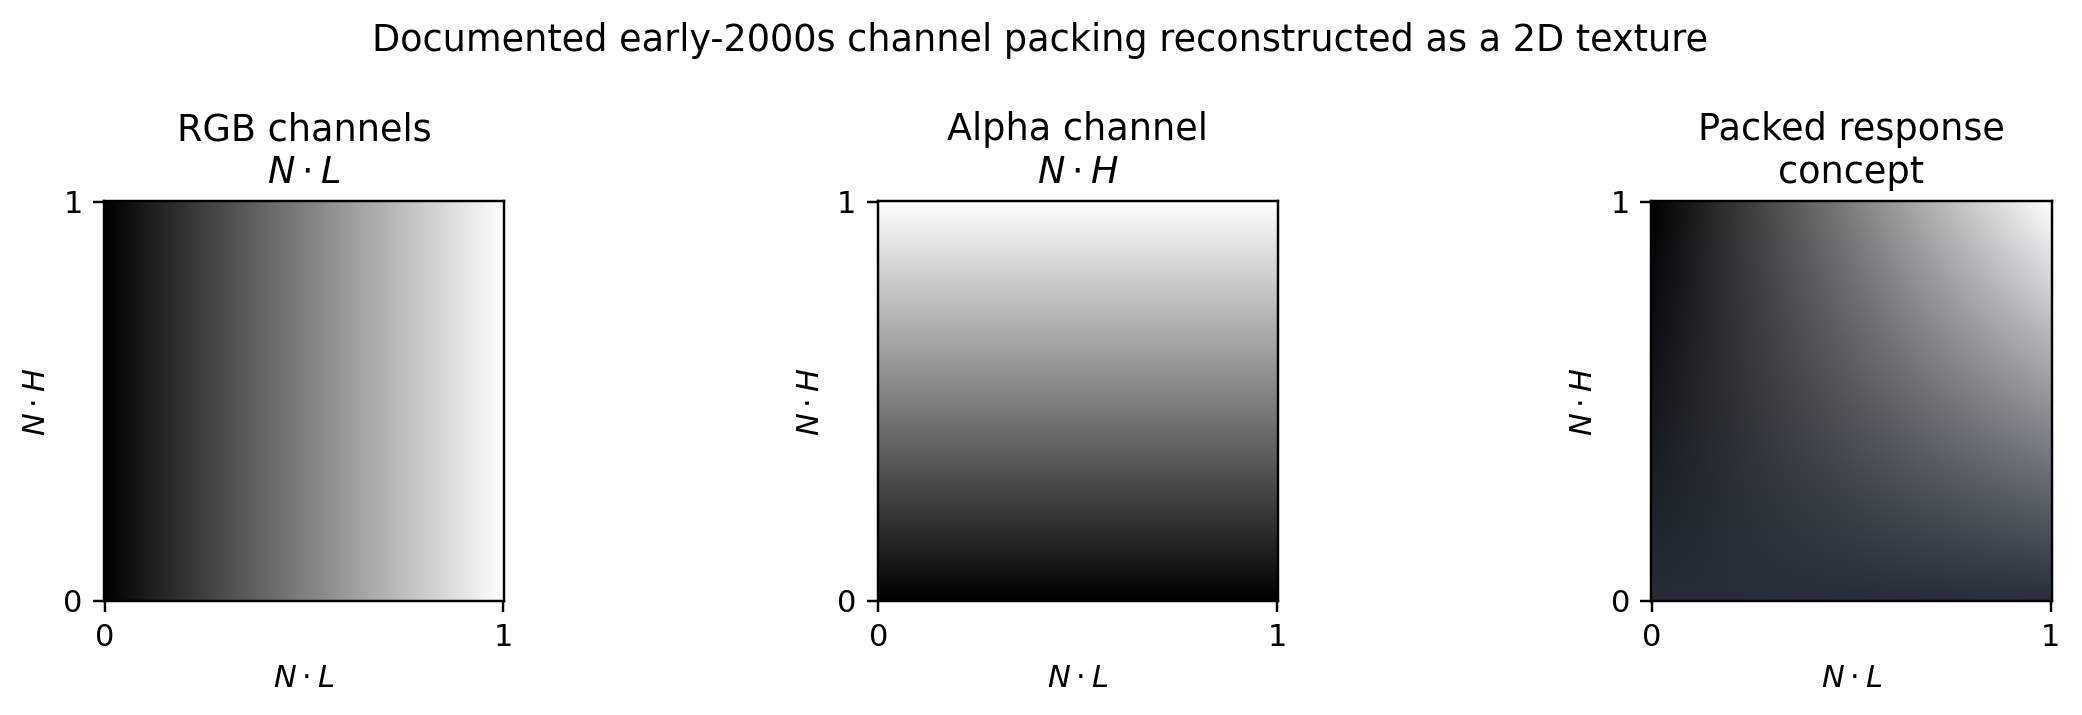
\includegraphics[width=0.92\linewidth]{figures/packed_response.png}
\caption{Reconstruction of the documented RGBA packing. This figure is generated from the surviving channel description; it is not an original NVEffectsBrowser texture.}
\label{fig:packed}
\end{figure}

This is deliberately conservative. It does not claim that the recovered texture format, filtering, exponent, or combine instructions are bit-identical to the original source.

\section{Why the Normal Map Matters}
A brushed finish has at least two visual scales:
\begin{enumerate}
\item the \textbf{aggregate lobe}, stretched because many microfacets share a preferred direction;
\item the \textbf{visible scratches/grooves}, which create high-frequency changes in normal, roughness, or both.
\end{enumerate}

The early shader page explicitly mentions a normal map, which addresses the second cue. Modern anisotropic BRDFs address the first. Treating them separately produces a more useful reconstruction than replacing the entire old method with one current ``brushed metal'' material preset.

The Unity package includes a deterministic directional normal-map generator. Its output is shown in Figure~\ref{fig:normal}.

\begin{figure}[H]
\centering
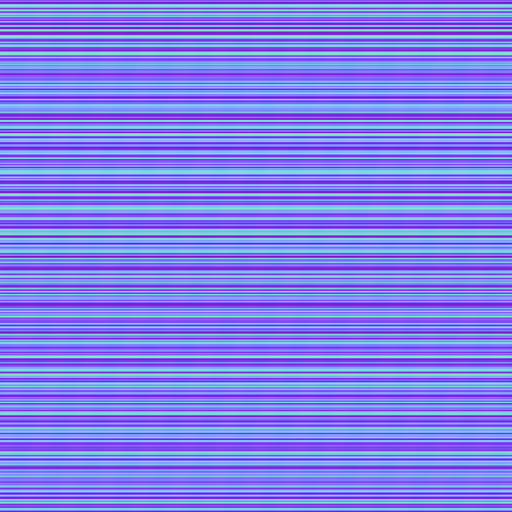
\includegraphics[width=0.58\linewidth]{figures/directional_brush_normal.png}
\caption{Generated directional brush normal map used by the historical and scratched-anisotropic modes.}
\label{fig:normal}
\end{figure}

\section{From Ward Anisotropy to Modern Microfacets}
Ward's 1992 reflectance model provided a practical analytic treatment of anisotropic reflection and validated it against measured surfaces \cite{ward1992}. Later models separated surface reflection into microfacet distribution, masking-shadowing, and Fresnel terms. GGX/Trowbridge-Reitz became widely used because of its long specular tails and practical behavior in physically based renderers \cite{walter2007}.

A modern anisotropic GGX normal-distribution function can be written
\begin{equation}
D(H)=\frac{1}{\pi\alpha_t\alpha_b\left[(T\cdot H/\alpha_t)^2+(B\cdot H/\alpha_b)^2+(N\cdot H)^2\right]^2},
\label{eq:aniso}
\end{equation}
where $T$ and $B$ define the material frame and $\alpha_t$, $\alpha_b$ are directional roughness values. Filament uses this form to explain why brushed metal requires anisotropic rather than isotropic reflection \cite{filament}.

Heitz showed that masking-shadowing must be consistent with the assumed microsurface distribution, and derived the stretch behavior needed for anisotropic Smith masking \cite{heitz2014}. Our reference implementation uses an anisotropic GGX distribution plus a Smith-style lambda term, which is substantially closer to a modern PBR material than the historical packed-dot response.

\begin{figure}[H]
\centering
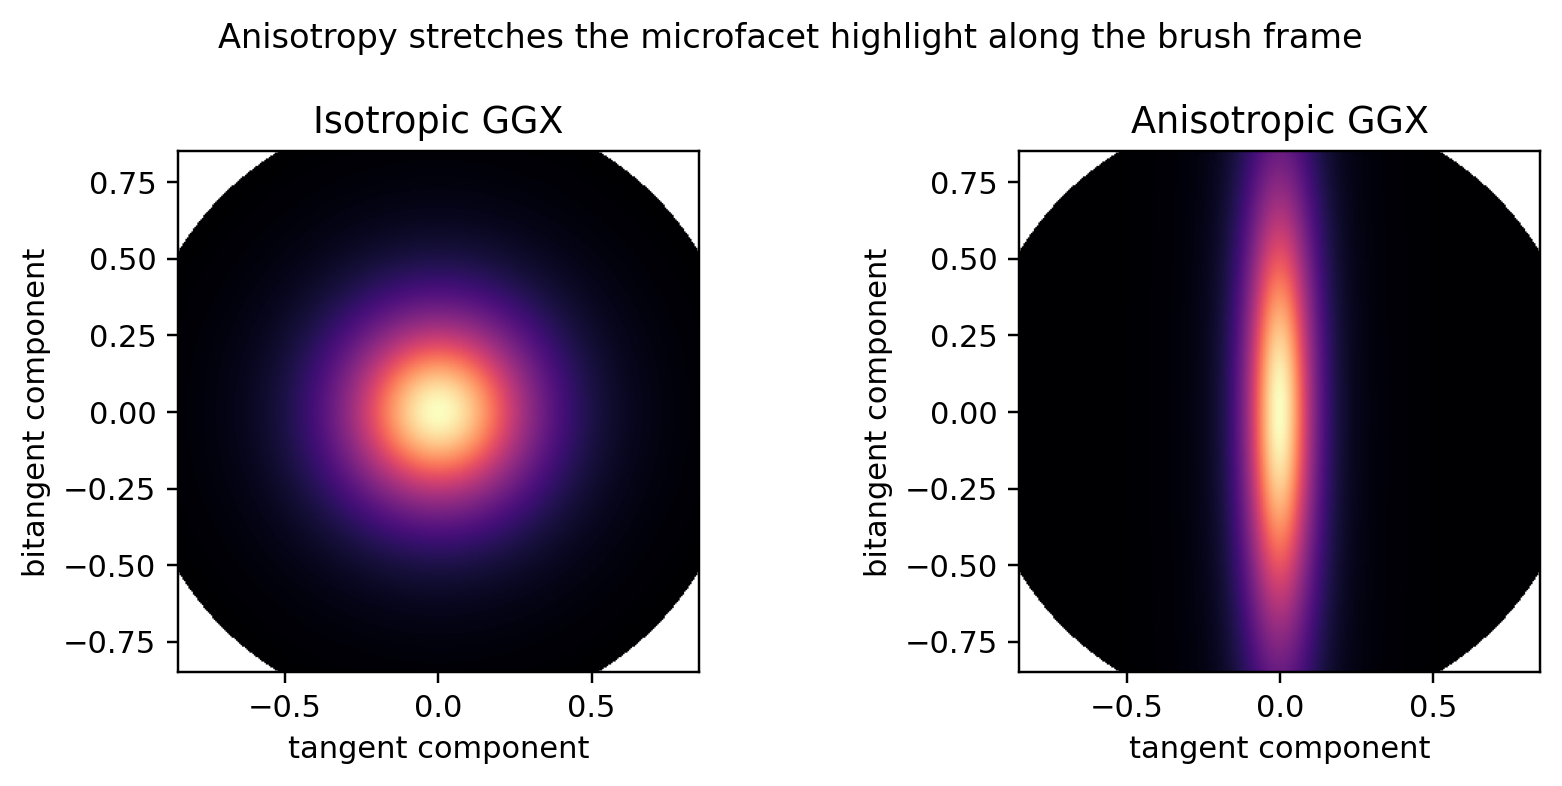
\includegraphics[width=0.78\linewidth]{figures/anisotropic_lobes.png}
\caption{Log-scaled GGX distribution over half-vector direction. Unequal tangent/bitangent roughness stretches the highlight in the local brush frame.}
\label{fig:lobes}
\end{figure}

\section{Unity 6 Reconstruction}
The package exposes four modes:

\begin{table}[H]
\centering
\small
\begin{tabular}{p{0.25\linewidth}p{0.68\linewidth}}
\toprule
\textbf{Mode} & \textbf{Purpose}\\
\midrule
Historical Packed & Samples the generated RGBA response from Equation~\ref{eq:packed} after a directional normal map, then applies a configurable Blinn-style exponent to alpha.\\
Isotropic GGX & Uses equal roughness in tangent and bitangent directions. This is the modern ``rough metal'' baseline.\\
Anisotropic GGX & Uses Equation~\ref{eq:aniso} with independent tangent and bitangent roughness.\\
Anisotropic + Scratches & Adds the generated brush normal map to the anisotropic model, separating lobe shape from visible microstructure.\\
\bottomrule
\end{tabular}
\caption{Reference material modes.}
\end{table}

The historical path makes the packed-data concept explicit:
\begin{lstlisting}[language=C]
float4 packed = SAMPLE_TEXTURE2D(_PackedResponseLUT, sampler_PackedResponseLUT,
                                float2(NoL, NoH));
float3 body = baseColor * packed.rgb;
float3 spec = baseColor * pow(packed.a, legacySpecularPower);
\end{lstlisting}

The modern path evaluates the anisotropic microfacet lobe directly. Metallic Fresnel is tinted by the metal base color, while the tangent frame controls highlight orientation.

\begin{figure}[H]
\centering
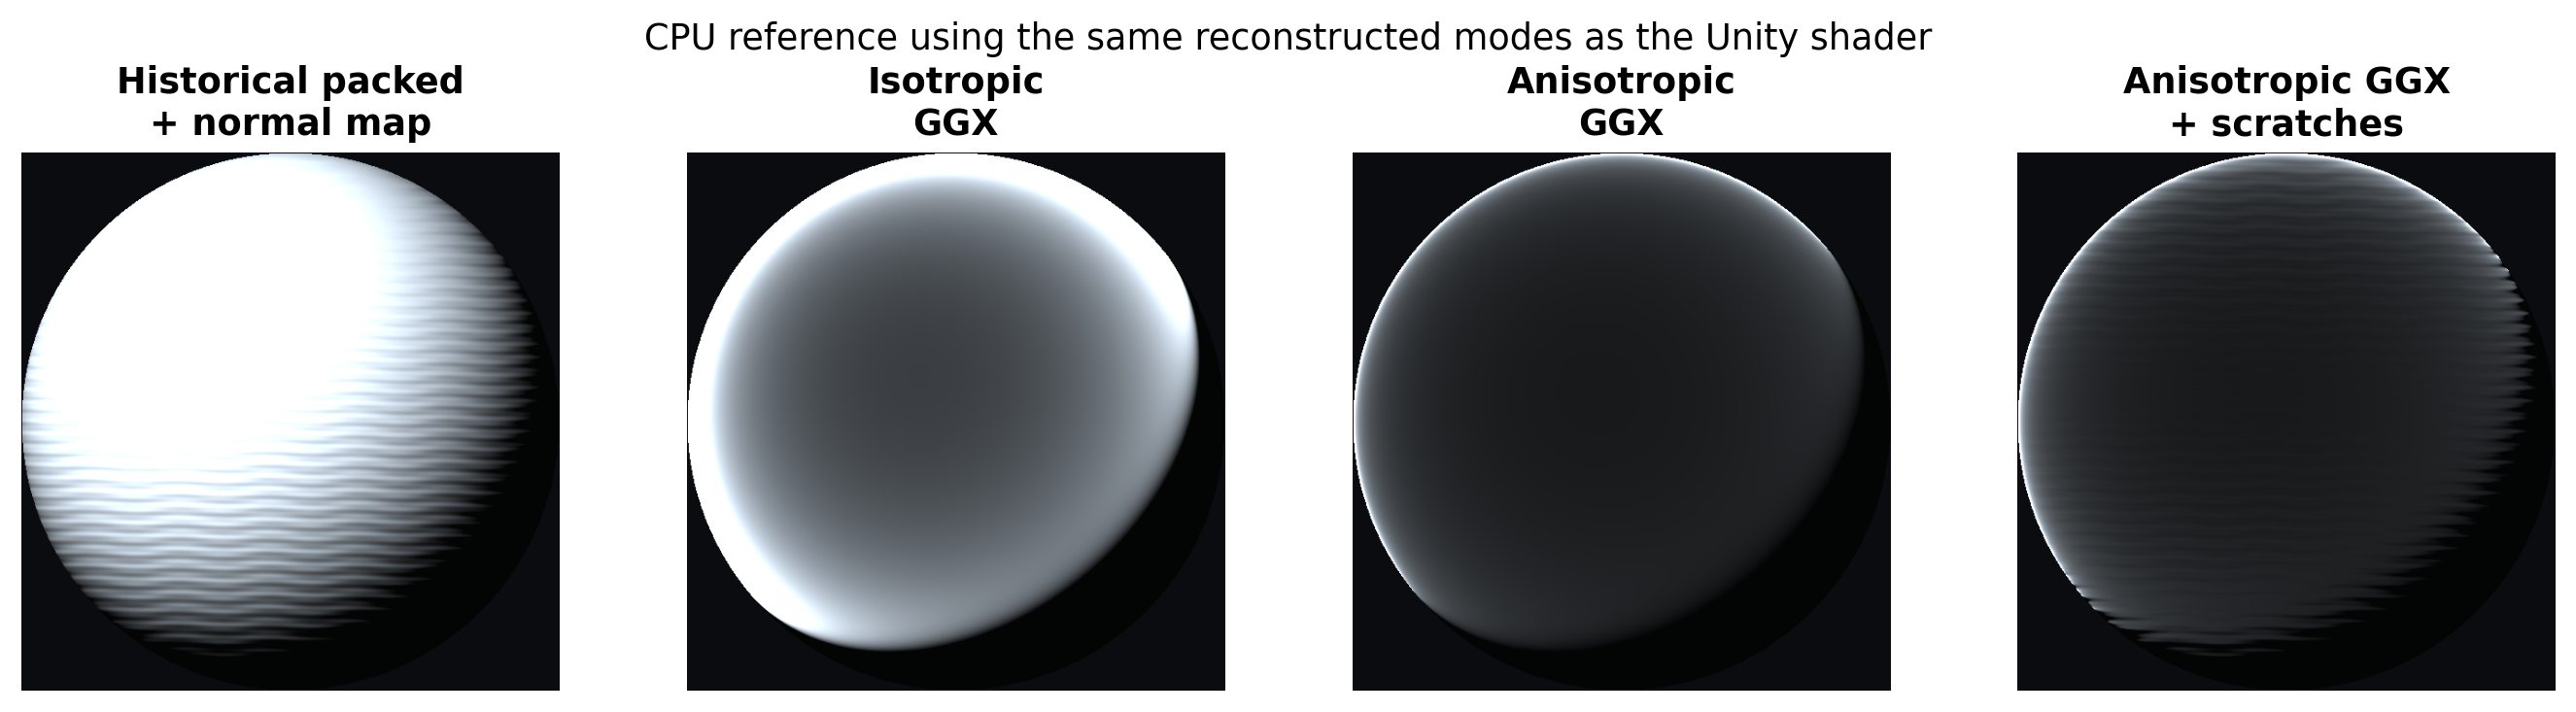
\includegraphics[width=\linewidth]{figures/brushed_mode_comparison.png}
\caption{CPU reference comparison using the same reconstructed modes and default parameters as the Unity package. These are diagnostic images, not Unity editor captures.}
\label{fig:modes}
\end{figure}

\section{Interpretation of the Historical Design}
The early shader is interesting even if anisotropic GGX is the preferred modern solution. Packing $N\cdot L$ and $N\cdot H$ into RGBA converts two common lighting inputs into data that texture and combiner hardware can carry together. On early pixel-shader hardware, this could reduce arithmetic, instruction pressure, and intermediate state.

The technique also highlights a broader transition in GPU programming. Around this period, textures were not merely images; they were tables for BRDFs, dot products, normalization, attenuation, and other functions. Hurley's contemporaneous GDC work explicitly framed textures as function storage rather than simple painted pixels, the same design philosophy visible in the Minnaert reconstruction.

\section{Relation to Period and Current Work}
Anisotropic reflection was already well established in offline rendering by the early 1990s \cite{ward1992}, and anisotropic Phong-family models were developed for efficient analytic shading \cite{ashikhmin2000}. What changed in the early 2000s was the amount of this work that commodity GPUs could perform per pixel.

NVIDIA's later Gelato shader documentation describes brushed metal as an anisotropic material caused by aligned microscopic grooves and notes that metal highlights inherit the metal color \cite{gelato2005}. Modern PBR engines express the same idea through tangent-space anisotropy. Filament, for example, states directly that materials such as brushed metal require an anisotropic model and uses anisotropic GGX \cite{filament}.

This does not make the old packed approach ``wrong.'' It makes it a compact implementation of a subset of the visual cues, shaped by a very different instruction and texture budget.

\section{Evaluation Plan}
The repository supports three types of evaluation:
\begin{enumerate}
\item \textbf{Appearance:} matched-lighting renders on spheres, cylinders, and planar appliance-like surfaces.
\item \textbf{Motion:} rotating the light and camera to test whether the highlight tracks the brush frame convincingly.
\item \textbf{Performance:} GPU timing for historical packed lookup, isotropic GGX, anisotropic GGX, and anisotropic plus scratch normal mapping.
\end{enumerate}

A useful perceptual study would ask viewers to rate ``brushed,'' ``polished,'' ``rough,'' and ``machined'' appearance without naming the shader. The expected comparison is not simply old versus new. It can separate how much recognition comes from lobe anisotropy, how much from visible scratches, and how much from the interaction of both.

\section{Limitations and Provenance}
The original Realistic3D page currently exposes its text reliably through search indexing, but the linked source ZIP and page image are intermittent on the legacy host. Therefore the historical channel semantics are well supported, while the exact original shader/combiner code is not yet recovered. This manuscript does not present reconstructed figures as original screenshots.

If the source ZIP is recovered later, the next step should be a line-by-line mapping from the old NVEffectsBrowser passes to the reconstruction and a preserved build of the original effect where licensing permits.

\section{Conclusion}
The brushed-metal effect shows a different facet of the same early-GPU craft as the Minnaert and refraction techniques: encode the expensive or awkward part of the lighting problem into texture data, then exploit the hardware's strongest operations. A modern anisotropic GGX shader is more general and more physically grounded, but the old packed $N\cdot L$ / $N\cdot H$ representation remains a compact historical example of data-driven shading. Preserving both in one test harness makes the evolution visible rather than merely replacing the old shader with a current material preset.

\begin{thebibliography}{99}
\bibitem{hurleybrushed} Kenneth Hurley. \emph{Brushed Metal}. Realistic3D, early 2000s. \url{https://www.realistic3d.com/brushed_metal.htm}
\bibitem{hurleypubs} Kenneth Hurley. Personal site, older source-code section listing the NVEffectsBrowser brushed-metal plug-in. \url{https://www.kennethhurley.com/}
\bibitem{ward1992} Gregory J. Ward. Measuring and Modeling Anisotropic Reflection. \emph{Computer Graphics (SIGGRAPH '92)}, 26(2):265--272, 1992. DOI: 10.1145/133994.134078.
\bibitem{ashikhmin2000} Michael Ashikhmin and Peter Shirley. An Anisotropic Phong BRDF Model. \emph{Journal of Graphics Tools}, 5(2), 2000.
\bibitem{walter2007} Bruce Walter, Stephen R. Marschner, Hongsong Li, and Kenneth E. Torrance. Microfacet Models for Refraction through Rough Surfaces. \emph{Eurographics Symposium on Rendering}, 2007.
\bibitem{heitz2014} Eric Heitz. Understanding the Masking-Shadowing Function in Microfacet-Based BRDFs. \emph{Journal of Computer Graphics Techniques}, 3(2):48--107, 2014. \url{https://jcgt.org/published/0003/02/03/}
\bibitem{filament} Google. Filament Physically Based Rendering Guide: Anisotropic Model. \url{https://google.github.io/filament/main/filament.html}
\bibitem{gelato2005} NVIDIA. Gelato Shader Library Documentation: \texttt{brushedmetal.gsl}, December 2005.
\end{thebibliography}
\end{document}
